\chapter{2023年「概率论 \& 数理统计」\titlelogo{https://sci.hdu.edu.cn}{HDU}期中回忆}

\date{2023年12月3日}{基础数学教学团队}{A0714040}
{未央数学讲师~ctz}
{https://qm.qq.com/q/OlkSiy9W04}{HDU 数学营}
{http://weixin.qq.com/r/mhKYgFTEMQlOrRDj90eI}{未央学社公众号}

\section{选择题（每题3分，共30分）}
\begin{choice}{C}
    已知$A$、$B$、$C$为三个随机事件，则$A$、$B$、$C$至少一个发生的事件为
\begin{tasks}(4)
    \task $\overline{ABC}$
    \task $\overline{ABC}$
    \task $A\cup B\cup C$
    \task $ABC$
\end{tasks}
\end{choice}

\begin{choice}{D}
    假设事件$A$和$B$满足$P(B|A)=1$，则
\begin{tasks}(4)
    \task $A$是必然事件
    \task $P(B|\overline{A})=0$
    \task $B\subset A$
    \task $A\subset B$
\end{tasks}
\end{choice}
\begin{solution}*
    $P(B|A)=1\Rightarrow\frac{P(AB)}{P(A)}=1\Rightarrow P(AB)=P(A)$，所以$A\subset B$. \sokka{D}
\end{solution}

\begin{choice}{D}
    在$100$以内的所有两位数中，任取一个数，则能被$2$或$3$整除的概率为
\begin{tasks}(4)
    \task $1/6$
    \task $1/4$
    \task $1/3$
    \task $2/3$
\end{tasks}
\end{choice}
\begin{solution}*
    能被$2$整除的概率为$45/90$，能被$3$整除的概率为$30/90$，能被$6$整除的概率为$15/90$，所以能被$2$或$3$整除的概率为$P=P(2)+P(3)-P(6)=\frac{45+30-15}{90}=\frac23$.
\end{solution}

\begin{choice}{C}
    随机变量$X$的期望$E(X)$存在，则$E[E(E(x))]=$
\begin{tasks}(4)
    \task $E^3(X)$
    \task $E^2(X)$
    \task $E(X)$
    \task 无法确定
\end{tasks}
\end{choice}
\begin{solution}*
    设$E(X)=a$，则$E[E(X)]=E(a)=a,\ E[E(E(X))]=E(a)=a=E(X)$. \sokka{C}
\end{solution}

\begin{choice}{B}
    任意两事件$A$和$B$，则下列关系正确的是
    \begin{tasks}(4)
        \task $(A-B)\cup B=A$
        \task $AB\cup(A-B)=A$
        \task $(A-B)-B=A$
        \task $(AB\cup A)-B=A$
    \end{tasks}
\end{choice}
\solute1
\begin{solution}
    \begin{tasks}(4)
        \task $(A-B)\cup B=A\cup B$
        \task* $AB\cup(A-B)=(A\cup(A-B))\cap(B\cup(A-B))=A\cap(A\cup B)=A$
        \task*(2) $(A-B)-B=(A-B)-(A-B)\cap B\neq A$
        \task*(2) $(AB\cup A)-B=A-B\neq A$
    \end{tasks}
\end{solution}

\begin{choice}{D}
    设随机变量$X$的概率密度为
    \[f(x)=\begin{cases}
        kx^2, & 0\leq x<2\\
        kx, & 2\leq x\leq 3\\
        0, & \text{else}
    \end{cases}\]
    则常数$k$的值为
    \begin{tasks}(4)
        \task $1/31$
        \task $3/31$
        \task $2/31$
        \task $6/31$
    \end{tasks}
\end{choice}
\solute3
\begin{solution}*
    归一化：$1=\int_0^2kx^2\d x+\int_2^3kx\d x=\frac{kx^3}{3}\Bigg|_0^2+\frac{kx^2}{2}\Bigg|_2^3=\frac{31}{6}k,\ k=\frac{6}{31}$. \sokka{D}
\end{solution}

\begin{choice}{B}
    设连续型随机变量$X$的概率密度函数和分布函数分别为$f(x)$和$F(x)$，则
    \begin{tasks}(4)
        \task $f(x)$可以是奇函数
        \task $f(x)$可以是偶函数
        \task $F(x)$可以是奇函数
        \task $F(x)$可以是偶函数
    \end{tasks}
\end{choice}
\begin{solution}*
    \begin{itemize}
        \item 由于$F(x)$为单调不减的连续函数，所以$F(x)$不是奇偶函数.
        \item 由于$f(x)$有正态分布函数$f(x)=\e^{-x^2/2}/\sqrt{2\pi}$，所以$f(x)$可以是偶函数. \sokka{B}
    \end{itemize}
\end{solution}

\begin{choice}{A}
    设随机变量$X$和$Y$都服从正态分布$N(0,\sigma^2)$，且$P(X\leq 1,Y\leq -1)=1/4$，则$P(X>1,Y>-1)$等于
\begin{tasks}(4)
    \task $1/4$
    \task $1/2$
    \task $3/4$
    \task $1/16$
\end{tasks}
\end{choice}
\solute3
\begin{solution}
\begin{itemize}
    \item $P(A)=P(X\leq q)=P\ab(\frac{X-0}{6}\leq\frac16)=\Phi\ab(\frac16)$.
    \item $P(B)=P(Y\leq -1)=P\ab(\frac{Y-0}{6}\leq-\frac16)=\Phi\ab(-\frac16)=1-\Phi\ab(\frac16)$.
    \item $P(X>1,Y>-1)=P(\overline{A}\overline{B})=P(\overline{A\cup B})=1-P(A)-P(B)+P(AB)=1-\Phi\ab(\frac16)-1+\Phi\ab(\frac16)+\frac14=\frac14$.
\end{itemize}
\end{solution}

\begin{choice}{C}
    设随机变量$X$的概率密度$f(x)$满足$f(1+x)=f(1-x)$，且$\int_0^2f(x)\d x=0.4$，则$P(X<0)$为
    \begin{tasks}(4)
        \task $0.1$
        \task $0.2$
        \task $0.3$
        \task $0.4$
    \end{tasks}
\end{choice}
\solute3
\begin{solution}*
\begin{itemize}
    \item 由于$f(1+x)=f(1-x)$，所以$f(x)$关于$X=1$对称，$P(x\leq 1)=P(x<1)=0.5$.
    \item 由于$P(0<x<2)=0.4$，所以$P(0<x<1)=0.2,\ P(x<0)=P(x<1)-P(0\leq x<1)=0.5-0.2=0.3$. \sokka{C}
\end{itemize}
\end{solution}


\begin{choice}{B}
    已知随机变量$X\sim B(n,p)$，且$E(X)=2.4,\ D(X)=1.44$，则参数$n,\ p$的值为
\begin{tasks}(4)
    \task $n=4,\ p=0.6$
    \task $n=6,\ p=0.4$
    \task $n=8,\ p=0.3$
    \task $n=24,\ p=0.1$
\end{tasks}
\end{choice}
\solute2
\begin{solution}*
    $E(X)=np=2.4$，$D(X)=np(1-p)=1.44$. 联立解得$n=6,\ p=0.4$. \sokka{B}
\end{solution}

\section{填空题（每题3分，共15分）}
\begin{problem}
    设随机变量$X,\ Y$相互独立，且有$E(X)=2,\ E(Y)=1,\ D(X)=D(Y)=1$，由切比雪夫不等式估计得$P(\abs{X-2Y}\geq5)=$\ans{$0.2$}.（结果用小数表示）
\end{problem}
\solute0
\begin{solution}
\begin{itemize}
    \item 设$Z=X-2Y$，所以$E(Z)=E(X)-2E(Y)=0,\ D(Z)=D(X)+4D(Y)=5$.
    \item $P(\abs{X-2Y}\geq5)\leq\frac{D(Z)}{5^2}=\frac15=0.2$.
\end{itemize}
\end{solution}

\begin{problem}
    随机变量$X$得概率密度为$f(x)=\begin{cases}
        2x, &0<x<1\\
        0, &\text{else}
    \end{cases}$，$Y$表示对$X$的三次独立重复观察中事件$(X\leq1/3)$出现的次数. 求$P(Y=2)=$\ans{$8/243$}（结果用分数表示）.
\end{problem}
\solute0
\begin{solution}
    由于$P\ab(X\leq\frac13)=\int_{-\infty}^{\frac13}f(x)\d x=\int_0^{\frac13}2x\d x=\frac19$，又$Y\sim B\ab(3,\frac19)$得$P(Y=2)=C_3^2\ab(\frac19)^2\cdot\frac89=\frac{8}{243}$.
\end{solution}

\begin{problem}
    设$X\sim\pi(1)$，则$F(2)=$\ans{$5/2\e$}.
\end{problem}
\begin{solution}*
    $F(2)=1/\e+1/\e+1/2\e=5/2\e$.
\end{solution}

\begin{problem}
    设事件$A,\ B,\ C$两两互斥，$P(A)=0.2,\ P(B)=0.3,\ P(C)=0.4$，则$P[(A\cup B)-C]=$\ans{$0.5$}.
\end{problem}
\begin{solution}*
\begin{itemize}
    \item $A\cap B=\varnothing,\ A\cap C=\varnothing,\ B\cap C=\varnothing\Rightarrow(A\cup B)\cap C=\varnothing$.
    \item $(A\cup B)-C=(A\cup B)-(A\cup B)\cap C=A\cup B$.
    \item $P[(A\cup B)-C]=P(A\cup B)=P(A)+P(B)-P(AB)=0.5$.
\end{itemize}
\end{solution}

\begin{problem}
    已知随机变量$X$服从参数为$2$的指数分布，则期望$E\ab(3\e^{-\frac x2}+1/2)=$\ans{$25/2$}.
\end{problem}
\solute0
\begin{solution}
    $P(x)=\begin{cases}
        2\e^{-2x}, & x>0\\
        0, & x\leq 0
    \end{cases}$，所以$E\ab(3\e^{-\frac x2}+\frac12)=\int_0^{+\infty}2\e^{-2x}\cdot\ab(3\e^{-\frac x2}+\frac12)\d x=\frac{25}{2}$.
\end{solution}

\section{计算题（共55分）}
\begin{problem}
设随机变量$X$和$Y$相互独立，且分布律如下
\begin{multicols}{2}
\centering
\begin{tabular}{c|cccc}
\toprule
    $X$ & 0 & 1 & 2 & 3\\
\hline
    $P$ & $1/3$ & $1/3$ & $1/6$ & $1/6$\\
\bottomrule
\end{tabular}

\begin{tabular}{c|ccc}
    \toprule
        $Y$ & -1 & 0 & 1\\
    \hline
        $P$ & $1/4$ & $1/2$ & $1/4$\\
    \bottomrule
    \end{tabular}
\end{multicols}
\columnseprule=.5pt
\begin{multicols}{2}
\begin{enumerate}
    \item 关于$X$和$Y$的联合分布律.
    \item 关于$XY$的分布律.
    \item $P(Y<1|X=0)$.
    \item $Cov(X-Y)$.
    \item $\rho_{XY}$.
\end{enumerate}
\end{multicols}
\end{problem}
\solute2
\begin{solution}
\columnseprule=.5pt
\begin{multicols}{2}
\begin{enumerate}
    \item 
    
    \begin{tabular}[t]{cccc}
    \toprule
        \diagbox{$Y$}{$X$}& $-1$ & $0$ & $1$\\
        \midrule
        \addlinespace[3pt]
        $0$ & $\frac{1}{12}$ & $\frac16$ & $\frac{1}{12}$\\
        \addlinespace[3pt]
        $1$ & $\frac{1}{12}$ & $\frac16$ & $\frac{1}{12}$\\
        \addlinespace[3pt]
        $2$ & $\frac{1}{24}$ & $\frac{1}{12}$ & $\frac{1}{24}$\\
        \addlinespace[3pt]
        $3$ & $\frac{1}{24}$ & $\frac{1}{12}$ & $\frac{1}{24}$\\
        \addlinespace[3pt]
    \bottomrule
    \end{tabular}
    \vskip1ex
    \item 令$Z=XY$，$Z$可取$-3,\ -2,\ -1,\ 0,\ 1,\ 2,\ 3$.
    
    \begin{tabular}{c|ccccccc}
        \toprule
        $Z$ & $-3$ & $-2$ & $-1$ & $0$ & $1$ & $2$ & $3$\\
        \hline
        $P$ & $\nicefrac{1}{24}$ & $\nicefrac{1}{24}$ & $\nicefrac{1}{12}$ & $\nicefrac23$ & $\nicefrac{1}{12}$ & $\nicefrac{1}{24}$ & $\nicefrac{1}{24}$\\
        \bottomrule
    \end{tabular}
    \vskip1ex
    \item 由于$X,\ Y$相互独立
    \[P\{Y<1|X=0\}=\frac12+\frac14=\frac34\]
    \item 由于$X,\ Y$相互独立
    \[\begin{aligned}
        Cov(X,-Y)&=E(-XY)-E(X)E(-Y)\\
        &=E(X)E(Y)-E(XY)=0
    \end{aligned}\]
    \item $\rho_{XY}=\frac{Cov(X,Y)}{\sqrt{D(X)}\sqrt{D(Y)}}$.
\end{enumerate}
\end{multicols}
\end{solution}

\begin{problem}
    有三个罐子，1号罐装有2红1黑共3个球，2号罐装有3红1黑共4个球，3号罐装有2红2黑共4个球. 某人从中随机取一罐，再从中任意取一球，已知取到是红球，问该红球取自1号罐的概率是多少？
\end{problem}
\solute2
\begin{solution}
    设事件$A$为取到红球，随机变量$X$表示取到第$X$号罐，$X=1,2,3$. 由题意得

\[\begin{cases}
    P\{A|X=1\}=\frac23\\
    P\{A|X=2\}=\frac34\\
    P\{A|X=3\}=\frac12\\
    P\{X=1\}=P\{X=2\}=P\{X=3\}=\frac13
\end{cases}\]
所以取到红球的概率为
\[P(A)=P\{A|X=1\}P\{X=1\}+P\{A|X=2\}P\{X=2\}+P\{A|X=3\}P\{X=3\}=\frac13\ab(\frac23+\frac34+\frac12)=\frac{23}{36}\]
该红球取自1号罐的概率是
\[P\{X>1|A\}=\frac{P\{X=1\cap A\}}{P(A)}=\frac{P\{A|X=1\}\cdot P\{X=1\}}{P(A)}=\frac{2/9}{23/36}=\frac{8}{23}\]
\end{solution}

\begin{problem}
    设离散型随机变量$X$的分布函数为
    \[F(X)=\begin{cases}
        0, & x<-1\\
        0.3, & -1\leq x<0\\
        0.8, & 0\leq x<1\\
        1, & x\geq 1
    \end{cases}\]
\begin{enumerate}
    \item $X$的概率分布律.
    \item $Y=X^2+1$的概率分布律.
    \item $D(Y+1)$.
\end{enumerate}
\end{problem}
\solute3
\begin{solution}
\begin{enumerate}
    \item $P\{X=-1\}=0.3,\ P\{X=0\}=0.8-0.3=0.5,\ P\{X=1\}=1-0.8=0.2$.
    \item $Y$可取$0,\ 1$. $P\{Y=0\}=P\{X=0\}=0.5,\ P\{Y=1\}=P\{X=1\cup X=-1\}=0.2+0.3=0.5$.

\begin{center}
    \begin{tabular}{c|cc}
        \toprule
        $Y$ & $0$ & $1$\\
        \midrule
        $P$ & $0.5$ & $0.5$\\
        \bottomrule
    \end{tabular}
\end{center}
    \item $Y\sim b(1,0.5),\ \begin{cases}
        n=1\\p=0.5
    \end{cases}$，所以$D(Y+1)=D(Y)=np(1-p)=0.25$.
\end{enumerate}
\end{solution}

\begin{problem}
    设二维随机变量$(X,Y)$的密度函数$f(x,y)=\begin{cases}
        2xy\e^{-x^2-y}, &x>0,y>0\\
        0, &\text{else}
    \end{cases}$. 已知$\int_{-\infty}^{+\infty}\e^{-x^2}\d x=\sqrt\pi$.
\columnseprule=.5pt
\begin{multicols}{2}
\begin{enumerate}
    \item 求$f_x(x)$和$f_y(y)$.
    \item $X$、$Y$是否相互独立？说明理由.
    \item 求$f_{Y|X}(y|x)$;
    \item 求$E(2X-Y)$.
\end{enumerate}
\end{multicols}
\end{problem}
\solute4
\begin{solution}
\begin{enumerate}
    \item $f_X(x)=\begin{cases}
        \int_{-\infty}^{+\infty}f(x,y)\d y=\int_0^\infty2xy\e^{-x^2-y}\d y\xlongequal{\text{Integration by parts}}2x\e^{-x^2} & x>0\\
        0 & x\leq 0
    \end{cases}$.

    $f_Y(y)=\begin{cases}
        \int_{-\infty}^{+\infty}f(x,y)\d x=\int_0^\infty y\e^{-y}\cdot2x\e^{-x^2}\d x\xlongequal{\text{Integration by parts}}y\e^{-y} & y>0\\
        0 & y\leq 0
    \end{cases}$.
    \item 当$x>0\cup y>0$时，$f(x,y)=2xy\e^{-x^2-y}=f_X(x)\cdot f_Y(y)$.
    
    当$x\leq 0\cup y\leq 0$时，$f(x,y)=0=f_X(x)\cdot f_Y(y)$. 所以$X$、$Y$相互独立.
    \item 由于$X$、$Y$相互独立，所以$f_{Y|X}(y|x)=f_Y(y)=\begin{cases}
        y\e^{-y}, & y>0\\
        0, & y\leq 0
    \end{cases}$.
    \item $\begin{aligned}[t]
        &E(X)=\int_{-\infty}^{+\infty}xf_X(x)\d x=\int_0^\infty2x^2\e^{-x^2}\d x=-x\e^{-x^2}\Big|_0^\infty+\int_0^\infty\e^{-x^2}\d x=\frac{\sqrt\pi}{2}\\
        &E(Y)=\int_{-\infty}^{+\infty}y^2\e^{-y}\d y=\int_0^\infty y^2\e^{-y}\d y=\ab(y^2\e^{-y}+2y\e^{-y}+2\e^{-y})\Big|_0^\infty=-2\\
        &E(2X-Y)=2E(X)-E(Y)=\sqrt\pi+2
    \end{aligned}$.
\end{enumerate}
\end{solution}

\begin{problem}
    设随机变量$(X,Y)$的密度函数为$f(x,y),\ x,y\in \mathbb{R}$. 令$Z=X-Y$，证明：$Z$的密度函数$f_Z(z)=\int_{-\infty}^{+\infty}(z+y,y)\d y$.
\end{problem}
\solute3
\begin{solution}
\begin{proof}*
    \[\begin{aligned}
        P(z<Z<z+\d z)&=P(z<X-Y<z+\d z)=\iint\limits_{z<X-Y<z+\d z}f_{X,Y}(x,y)\d x\d y\\
        &\xlongequal[v=y]{u=x-y}f_Z(z)\d z=\int_{-\infty}^{+\infty}\int_z^{z+\d z}f_{X,Y}(u+v,v)\d u\d v
    \end{aligned}\]
利用$\int_z^{z+\d z}f_{X,Y}(u+v,v)\d u=\d z\cdot f(z+v,v)$得
\[f_Z(z)\d z=\int_{-\infty}^{+\infty}f(z+v,v)\d v=\int_{-\infty}^{+\infty}f(z+y,y)\d y\eqno\text{\QED}\]
\end{proof}
\end{solution}


\vfill
\rightline{/*Powered by \pkg{LiteSolution} \textsf\LaTeX~Template. Designed by WeYoung \href{https://ctan.org/home/xiamyphys}{Axia}.*/}

\newpage

\begin{tcolorbox}[blanker,
    left=3mm,
    toprule=.3em,
    bottomrule=.3em,
    bottomtitle=.75\baselineskip,
    fonttitle=\bfseries,
    borderline west={1.5pt}{0mm}{teal},
    coltitle=teal,sidebyside,righthand width=\dimeval{2\textwidth/7}]
    \lipsum[2]
    \tcblower\centering
    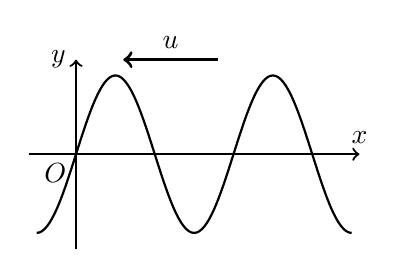
\begin{tikzpicture}
        \draw [thick,->] (-0.6,0)--(3.6,0) node [anchor=south] {$x$};
        \draw [thick,->] (0,-1.2)--(0,1.2) node [anchor=east] at (0,1.2) {$y$};
        \draw [thick] (-0.5,-1) cos (0,0) sin (0.5,1) cos (1,0) sin (1.5,-1) cos (2,0) sin (2.5,1) cos (3,0) sin (3.5,-1);
        \node [anchor=north east] at (0,0) {$O$};
        \draw [very thick,<-] (0.6,1.2)--(1.8,1.2) node [anchor=south,midway] {$u$};
    \end{tikzpicture}
\end{tcolorbox}